\documentclass[11pt]{article}

%%%%%%%%%%%%
% Packages %
%%%%%%%%%%%%

\hyphenpenalty=10000
\usepackage{tikz}
\usetikzlibrary{shapes,arrows}


\usepackage{tocloft}
\renewcommand\cftsecleader{\cftdotfill{\cftdotsep}}
\def\undertilde#1{\mathord{\vtop{\ialign{##\crcr
$\hfil\displaystyle{#1}\hfil$\crcr\noalign{\kern1.5pt\nointerlineskip}
$\hfil\tilde{}\hfil$\crcr\noalign{\kern1.5pt}}}}}
\usepackage{cleveref}
\usepackage{xcolor}
\usepackage[colorlinks = true,
            linkcolor = black,
            urlcolor  = black,
            citecolor = black,
            anchorcolor = black]{hyperref}
\usepackage{epstopdf}
\usepackage{braket}
\usepackage{upgreek}
\usepackage{caption}
\usepackage{booktabs}
\usepackage{subcaption}
\usepackage{amssymb,latexsym,amsmath,gensymb}
\usepackage{latexsym}
\usepackage{graphicx}
\usepackage{float}
\usepackage{enumitem}
\usepackage{pdflscape}
\usepackage{url}
\usepackage{array}
\newcolumntype{C}{>{$\displaystyle} c <{$}}
\usepackage{tikz, calc}
\usetikzlibrary{shapes.geometric, arrows, calc}
\tikzstyle{norm} = [rectangle, rounded corners, minimum width=2cm, minimum height=1cm,text centered, draw=black]
\tikzstyle{arrow} = [thick, ->, >=stealth]

\newcommand{\argmin}{\arg\!\min}
\newcommand{\me}{\mathrm{e}}
\providecommand{\e}[1]{\ensuremath{\times 10^{#1}}} 
\providecommand{\mb}[1]{\mathbf{#1}}
\providecommand{\mf}[1]{\mathfrak{#1}}
\providecommand{\ro}[1]{\mathbf{\mathfrak{r}}_o}
\providecommand{\so}[1]{\mathbf{\hat{s}}_o}
\providecommand{\rb}[1]{\mathbf{r}_b}
\providecommand{\rbm}[1]{r_b^{\text{m}}}
\providecommand{\rd}[1]{\mathbf{r}_d}
\providecommand{\mh}[1]{\mathbf{\hat{#1}}}
\providecommand{\bs}[1]{\boldsymbol{#1}} 
\providecommand{\intinf}{\int_{-\infty}^{\infty}}
\providecommand{\fig}[4]{
  % filename, width, caption, label
\begin{figure}[h]
 \captionsetup{width=1.0\linewidth}
 \centering
 \includegraphics[width = #2\textwidth]{#1}
 \caption{#3}
 \label{fig:#4}
\end{figure}
}

\newcommand{\tensor}[1]{\overset{\text{\tiny$\leftrightarrow$}}{\mb{#1}}}
\newcommand{\tunderbrace}[2]{\underbrace{#1}_{\textstyle#2}}
\providecommand{\figs}[7]{
  % filename1, filename2, caption1, caption2, label1, label2, shift
\begin{figure}[H]
\centering
\begin{minipage}[b]{.45\textwidth}
  \centering
  \includegraphics[width=1.0\linewidth]{#1}
  \captionsetup{justification=justified, singlelinecheck=true}
  \caption{#3}
  \label{fig:#5}
\end{minipage}
\hspace{2em}
\begin{minipage}[b]{.45\textwidth}
  \centering
  \includegraphics[width=1.0\linewidth]{#2}
  \vspace{#7em}
  \captionsetup{justification=justified}
  \caption{#4}
  \label{fig:#6}
\end{minipage}
\end{figure}
}
\makeatletter

\providecommand{\code}[1]{
\begin{center}
\lstinputlisting{#1}
\end{center}
}

\newcommand{\crefrangeconjunction}{--}
%%%%%%%%%%%
% Spacing %
%%%%%%%%%%%
% Margins
\usepackage[
top    = 1.5cm,
bottom = 1.5cm,
left   = 1.5cm,
right  = 1.5cm]{geometry}

% Indents, paragraph space
%\usepackage{parskip}
\setlength{\parskip}{1.5ex}

% Section spacing
\usepackage{titlesec}
\titlespacing*{\title}
{0pt}{0ex}{0ex}
\titlespacing*{\section}
{0pt}{0ex}{0ex}
\titlespacing*{\subsection}
{0pt}{0ex}{0ex}
\titlespacing*{\subsubsection}
{0pt}{0ex}{0ex}

% Line spacing
\linespread{1.1}

%%%%%%%%%%%%
% Document %
%%%%%%%%%%%%
\begin{document}
\title{\vspace{-2.5em} Spatio-angular transfer functions for fluorescence microscopes\vspace{-1em}}  \author{Talon Chandler, Min Guo, Hari Shroff, Rudolf Oldenbourg, Patrick La Rivi\`ere}
\date{\vspace{-1em}\today\vspace{-1em}}
\maketitle
\begin{abstract}
  We investigate how the orientation and position of fluorescent dipole emitters
  affects microscopic imaging using electromagnetic optics theory. Starting with
  the thoroughly studied spatio-angular point spread function, we introduce the
  spatio-angular coherent spread function, coherent transfer function, and
  optical transfer function as electromagnetic extensions of well-known
  functions in scalar optics theory. We use these concepts to show that
  fluorescence microscopes have a spatio-angular band limit. Finally, we study
  polarized light microscopes and find that polarized illumination is a type of
  structured illumination that extends the angular band limit.
\end{abstract}
\section{Introduction}
TODO

We use plain roman type for scalars, e.g., $x, y, z$; bold lowercase roman type
for two-dimensional vectors, e.g., $\mb{r}$; hats for unit vectors, e.g.,
$\mb{\hat{s}}$; bold lowercase gothic type for three-dimensional vectors, e.g.,
$\mb{\mathfrak{r}}$; and bold capital roman type for matrices, e.g.,
$\mb{R}$. We use the real spherical harmonic functions
\begin{align}
  y_l^m(\theta, \phi) =
  \begin{cases}
    \sqrt{2}K_l^m\cos(m\phi)P_l^m(\cos\theta), & m > 0\\
    K_l^0P_l^0(\cos\theta), & m = 0\\
    \sqrt{2}K_l^m\sin(-m\phi)P_l^{-m}(\cos\theta), & m < 0\\
  \end{cases}
\end{align}
where
\begin{align}
  K_l^m = \sqrt{\frac{(2l+1)}{4\pi}\frac{(l-|m|)!}{(l+|m|)!}},
\end{align}
and $P_l^m(x)$ are the associated Legendre polynomials. The $l=0$ and $l=1$
spherical harmonics are given by
\begin{equation}
\begin{aligned}
  y_0^0(\theta, \phi) &= \sqrt{\frac{1}{4\pi}},\\
  y_1^{-1}(\theta, \phi) = \sqrt{\frac{3}{4\pi}}\sin\phi\sin\theta, \hspace{2em} y_1^0(\theta, \phi) &= \sqrt{\frac{3}{4\pi}}\cos\theta, \hspace{2em} y_1^1(\theta, \phi) = \sqrt{\frac{3}{4\pi}}\cos\phi\sin\theta.
\end{aligned}
\end{equation}

\section{General forward model}
Consider a three-dimensional field of oriented fluorescent dipoles. We can
represent the entire field using a function $f(\ro{}, \so{})$ that returns the
number of dipoles at position $\ro{}$ per unit volume oriented in direction
$\so{}$ per unit solid angle. We call $f(\ro{}, \so{})$ the fluorescence
spatio-angular density because it has units of fluorophores per volume per solid
angle.

If each fluorophore in the field fluoresces independently then the measured
intensity is a weighted sum of the intensity contributions from each
fluorophore, and we can model the imaging system with
\begin{align}
  g_i(\rd{}) = \int_{\mathbb{R}^3}d\ro{} \int_{\mathbb{S}^2}d\so{}\ h_i(\rd{}; \ro{}, \so{})f(\ro{}, \so{})\label{eq:forward}
\end{align}
where $g_i(\mb{r_d})$ are the intensities measured by the detector under the
$i$th measurement configuration ($i$ can index polarizer settings or views),
$\mb{r_d}$ is the two-dimensional detector coordinate, and
$h_i(\rd{}; \ro{}, \so{})$ is the spatio-angular point spread function (PSF) of
the $i$th measurement configuration. Our goal is to reconstruct the object
$f(\ro{}, \so{})$ from intensity measurements $g_i(\rd{})$.

We can also use the spatio-angular density to model translating and rotating
fluorophores. As long as each fluorescence emission is an independent event,
then equation \ref{eq:forward} is a valid way to model the imaging system.

\section{Spatio-angular point spread function}
\begin{figure}[h]
 \captionsetup{width=1.0\linewidth}
 \centering
   \centering
   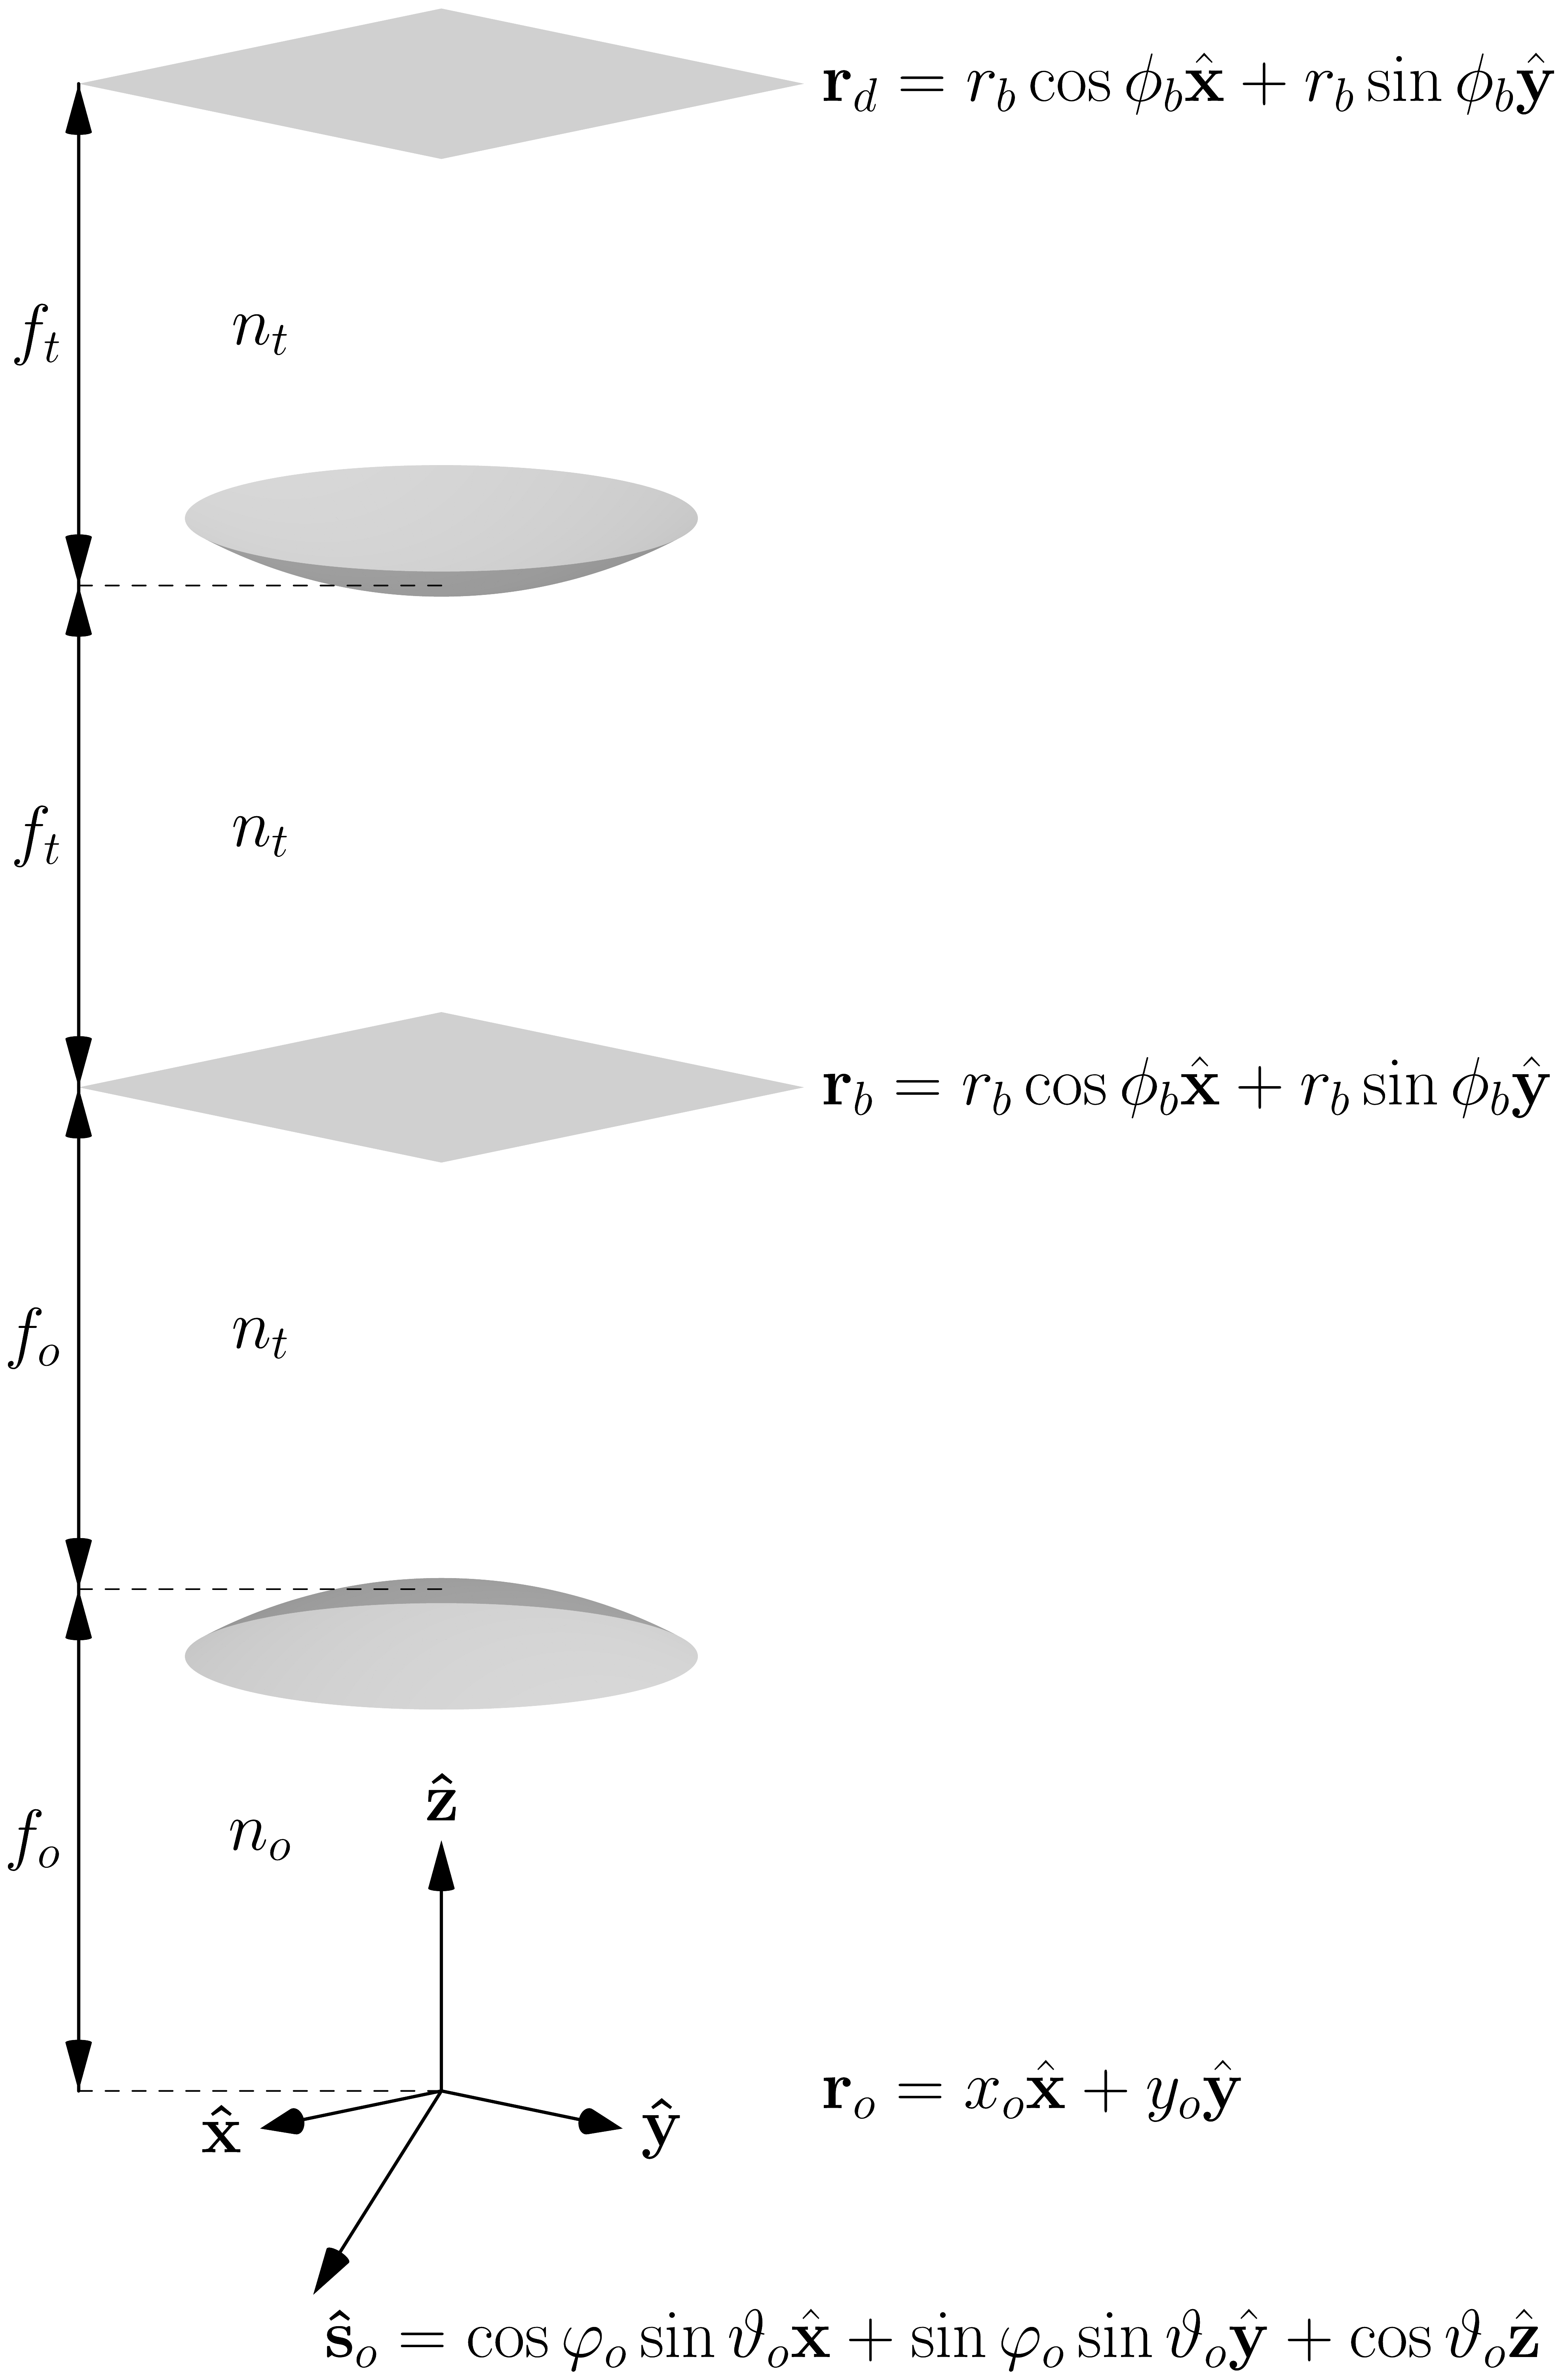
\includegraphics[width = 0.4\textwidth]{../figures/schematic.pdf}
   \caption{Simplified schematic of a single-view fluorescence microscope. The
     object is placed near the focal point of an aplanatic objective lens with
     focal length $f_{o}$ in a medium with refractive index $n_o$. The object is
     parameterized by the 3D position vector $\ro{}$ ($o$ for object) and an
     orientation unit vector $\so{}$. The light emitted by the fluorescent
     object is collected and collimated by the objective lens so that the
     electric fields are purely transverse in the back focal plane. Points in
     the back focal plane are parameterized by a 2D position vector $\rb{}$ ($b$
     for back focal plane). Finally, the tube lens with focal length $f_t$
     refocuses the light onto a detector. Points on the detector are
     parameterized by a 2D position vector $\rd{}$ ($d$ for detector). The back
     focal plane and detector are in a medium with refractive index $n_t$. Note
     that this schematic is not to scale---we consider the case where
     $f_o \ll f_t$.}
   \label{fig:frames_a}
\end{figure}

Figure \ref{fig:frames_a} shows a schematic of the fluorescence microscope that
we are considering with a summary of our notation. We start by following Backer
and Moerner \cite{backer2014} to find the electric field in the back focal plane
due to a single dipole emitter at position $\ro{}$ oriented along $\so{}$ as 
\begin{align}
  \mb{e_b}(\rb{};\ro{}, \so{}) \propto \me^{in_ok(z_o\rho_b)}\sqrt{\frac{1}{\rho_b}}
  \begin{bmatrix}
    \sin^2\phi_b + \rho_b\cos^2\phi_b&\sin\phi_b\cos\phi_b(\rho_b - 1)&-r_b\cos\phi_b\\
    \sin\phi_b\cos\phi_b(\rho_b - 1)&\cos^2\phi_b + \rho_b\sin^2\phi_b&-r_b\sin\phi_b\\
    0&0&0
  \end{bmatrix}
  \begin{bmatrix}
    \cos\varphi_o\sin\vartheta_o\\
    \sin\varphi_o\sin\vartheta_o\\
    \cos\vartheta_o
  \end{bmatrix}
\Pi\left(\frac{r_b}{r_b^{\text{max}}}\right)\label{eq:bfp}
\end{align}
where $r_b$ is the distance from the center of the back focal plane in units of
$f_o$, we define $\rho_b \equiv \sqrt{1 - r_b^2}$, and $\Pi(x)$ is a boxcar
function that returns 1 when $|x| < 1$ and 0 otherwise. We can understand this
expression term by term---the exponential term accounts for the defocus phase,
the square root term conserves power before and after the objective lens, the
matrix models the dipole emission process and electric field rotation caused by
the objective lens, the vector is the dipole orientation unit vector, and
$\Pi\left(\frac{r_b}{r_b^{\text{max}}}\right)$ accounts for the numerical
aperture of the lens with $r_b^{\text{max}} = \frac{f_0}{n_0}\text{NA}$. Notice
that we have omitted the dependence on the transverse position of the
fluorophore $x_o$ and $y_o$. This is because we assume that the objective is
aplanatic, so it displays transverse shift-invariance and the constant phase
factor does not affect our discussion.

We can find the intensity in the detector plane by propagating the electric
field to the detector plane using a scaled Fourier transform then taking the
modulus squared
\begin{align}
  h_i(\rd{}; \ro{}, \so{}) = \left|\int_{\mathbb{R}^2} d\rb{} \mb{e}_b(\rb{}; \ro{}, \so{})\me^{-i (kn_t/f_t) \rb{} \cdot \rd{}}\right|^2 \label{eq:kernel}.
\end{align}
Following Novotny \cite{nov2006}, we write the Fourier transform in polar
coordinates, evaluate the azimuthal integrals, and write the result concisely in
terms of three radial integrals
\begin{align}
    h_i(\rd{}; \ro{}, \so{}) &= \left|\mb{e}_d(\rd{}; \ro{}, \so{})\right|^2 \label{eq:kernel2}.\\
  \mb{e}_d(\rd{}; \ro{}, \so{}) &\propto
  \begin{bmatrix}
    I_0 + I_2\cos(2\phi_d) & I_2\sin(2\phi_d) & -2iI_1\cos\phi_d\\
    I_2\sin(2\phi_d) & I_0 - I_2\cos(2\phi_d) & -2iI_1\sin\phi_d\\
    0&0&0\\
  \end{bmatrix}
  \begin{bmatrix}
    \cos\varphi_o\sin\vartheta_o\\
    \sin\varphi_o\sin\vartheta_o\\
    \cos\vartheta_o
  \end{bmatrix}\label{eq:elec}
\end{align}
where $I_0, I_1$ and $I_2$ are
\begin{align}
  I_0(r_d; z_o) &= \int_0^{\theta_{\text{max}}}d\theta\ \sqrt{\cos\theta}\sin\theta(1+\cos\theta)J_0(k_b r_d\sin\theta f_o/f_t)\ \text{exp}\left\{ik_bz_o[1-(1/2)(f_o/f_t)^2\sin^2\theta]\right\},\\
  I_1(r_d; z_o) &= \int_0^{\theta_{\text{max}}}d\theta\ \sqrt{\cos\theta}\sin^2\theta J_1(k_b r_d\sin\theta f_o/f_t)\ \text{exp}\left\{ik_bz_o[1-(1/2)(f_o/f_t)^2\sin^2\theta]\right\},\\
  I_2(r_d; z_o) &= \int_0^{\theta_{\text{max}}}d\theta\ \sqrt{\cos\theta}\sin\theta(1-\cos\theta)J_2(k_b r_d\sin\theta f_o/f_t)\ \text{exp}\left\{ik_bz_o[1-(1/2)(f_o/f_t)^2\sin^2\theta]\right\}.
\end{align}
By plugging Eq. \ref{eq:elec} into equation Eq. \ref{eq:kernel2} and expanding in
terms of the spherical harmonic functions, we can rewrite the spatio-angular
PSF as
\begin{equation}
  \begin{split}
  h(\rd{}; \ro{}, \so{}) \propto &\left(I_0^2 + 2I_1^2 + I_2^2\right)y_0^0(\so{}) -\frac{2\sqrt{15}}{5}I_0I_2\sin(2\phi_d)y_2^{-2}(\so{})\\ &+ \frac{1}{\sqrt{5}}\left(-I_0^2 + 4I_1^2 - I_2^2\right)y_2^{0}(\so{}) +\frac{2\sqrt{15}}{5}I_0I_2\cos(2\phi_d)y_2^{2}(\so{}). \label{eq:kerna}
\end{split}
\end{equation}

We have chosen to write the spatio-angular PSF in terms of spherical harmonic
functions for two reasons. First, it allows us to express the spatio-angular PSF
very concisely. Instead of considering the point spread function for every
possible dipole orientation, we only need to consider four spatio-angular
PSFs---one for each spherical harmonic. Second, the spherical harmonic functions
form an orthonormal basis for functions on the sphere---a convenient fact that
we will use later.

It is useful to compare equation \ref{eq:kerna} to Backer and Moerner's approach
\cite{backer2014}. They expand the spatio-angular PSF in terms of six second
moments of the fluorophore distribution
$\{s_x^2, s_y^2, s_z^2, s_xs_y, s_xs_z, s_ys_z\}$. This approach is very
useful---only six precomputed spatio-angular PSFs are required to represent an
arbitrary spatio-angular PSF. Instead of expanding in terms of six second
moments, we expand onto just four spherical harmonics which, unlike the second
moments, are orthonormal functions. In the next section we will use the
orthonormality of the spherical harmonics to derive spatio-angular transfer
functions for fluorescence microscopes.

For now, let's look closer at the spatio-angular PSF in a special case. By
constraining the object to the focal plane ($z_o$ = 0) and applying the paraxial
approximation ($\sin\theta\approx\theta$ and $\cos\theta\approx 1$), the
integrals $I_{0-2}$ can be evaluated in terms of Bessel functions. We can
evaluate $I_0$ and $I_1$ with the help of $\int_0^zdx\ xJ_0(ax) = zJ_1(az)/a$
and $\int_0^zdx\ x^2J_1(ax) = z^2J_2(az)/a$, respectively, and $I_2 = 0$ because
$J_2(x)$ is zero to first order. In this case, the spatio-angular PSF simplifies
to
\begin{align}
      \lim_{\theta_{\text{max}} \ll \pi/2} h(\rd{}; \mathbf{r}_o, z_o=0, \so{}) \equiv h^{(p)}(\rd{}; \mathbf{r}_o, \so{}) \propto \left({I_0^{(p)}}^2 + 2{I_1^{(p)}}^2\right)y_0^0(\so{}) + \frac{1}{\sqrt{5}}\left(-{I_0^{(p)}}^2 + 4{I_1^{(p)}}^2\right)y_2^{0}(\so{})\label{eq:para}
\end{align}
where the integrals evaluate to
\begin{align}
  {I_0^{(p)}} = \left[\frac{2J_1(\tilde{r}_d)}{\tilde{r}_d}\right],
  \hspace{2em}
    {I_1^{(p)}} = \frac{\text{NA}}{n_o}\left[\frac{2J_2(\tilde{r}_d)}{\tilde{r}_d}\right],
  \intertext{and we have substituted}
  \tilde{r}_d = \frac{2\pi\text{NA}\thinspace r_d}{M\lambda},\hspace{2em}
  \text{NA} = n_o\sin\theta_{\text{max}},\hspace{2em}
  M = \frac{n_o}{n_b}\frac{f_t}{f_o}.
\end{align}
We will continue to use an superscipt $(p)$ to mark the terms where we have used
the paraxial approximation and constrained the object to the focal plane.
    
First, consider the coefficient on the $y_0^0$ spherical harmonic in
Eq. \ref{eq:para}. This coefficient is the point spread function for a angularly
uniform distribution of fluorophores. The first term of the coefficient $I_0^{(p)}$
is the familiar Airy disk that arises from the contribution of dipoles oriented
in the transverse plane, while the second term $I_1^{(p)}$ is a smaller factor that
arises from dipoles oriented outside of the transverse plane. This leads to an
interesting conclusion---a uniform distribution of dipoles has a point spread
function that is slightly wider than an Airy disk even in the paraxial
approximation. The Airy disk is usually derived using paraxial scalar optics
while here we have used paraxial electromagnetic optics. Therefore, we can
consider the second term to be an electromagnetic correction to the Airy
disk. We will quantify this difference in the next section.

Next, consider the coefficient on the $y_2^0$ spherical harmonic in
Eq. \ref{eq:para}. This coefficient is the spatial PSF for a distribution of
fluorophores proportional to $3\cos^2\vartheta_o - 1$. Counterintuitively, this
fluorophore distribution cannot exist because it would require a negative number
of fluorophores along some orientations; but if this distribution could exist,
then this coefficient would be its spatial PSF. Considering negative
distributions of fluorophores in our calculations should not be cause for
concern. The spherical harmonics span the space of functions on the sphere, so
any positive fluorophore distribution can be represented by the spherical
harmonics and we never need to consider negative fluorophores.
    
Finally, consider all of the spherical harmonics that have a zero
coefficient. These spherical harmonics span the angular null space of our
measurement system---fluorophore distributions that lie in the null space do not
affect the measured intensities. Under the paraxial approximation all of the
non-zero coefficients are rotationally symmetric ($m=0$) spherical harmonics
which means that the transverse orientation of the dipoles does not affect the
PSF. In the high NA case this is no longer true---two $m=2$ spherical harmonics
have non-zero coefficients and the transverse orientation of dipoles does affect
the PSF.


\section{Spatio-angular transfer functions}
We define the spatio-angular optical transfer function (OTF) as
\begin{align}
  H_l^m(\bs{\nu}_o) = \int_{\mathbb{R}^3}d\ro{} \int_{\mathbb{S}^2}d\so{}\ h_i(\rd{}; \ro{}, \so{}) y_l^m(\so{})\thinspace\me^{i 2\pi \ro{}\cdot\bs{\nu}_o}. \label{eq:ft}
\end{align}
The spatio-angular OTF measures the ability of the microscope to pass
spatio-angular harmonics---instead of the usual spatial harmonics
$\me^{i 2\pi \ro{}\cdot\bs{\nu}_o}$ we now need consider the spatio-angular
harmonics $y_l^m(\so{})\thinspace\me^{i 2\pi
  \ro{}\cdot\bs{\nu}_o}$. Eq.~\ref{eq:ft} can be interpreted as the
spatio-angular Fourier transform of the spatio-angular PSF.

We can plug Eq. \ref{eq:kerna} into \ref{eq:ft} and use the orthonormality
relation for spherical harmonics $\int_{\mathbb{S}^2}d\so{} y_{l_0}^{m_0}(\so{})y_{l_1}^{m_1}(\so{}) = \delta(l_0 - l_1, m_0 - m_1)$ to find that
\begin{equation}
  \begin{split}
  H_l^m(\bs{\nu}_o) \propto \int_{\mathbb{R}^3}d\ro{}  \bigg[&\left(I_0^2 + 2I_1^2 + I_2^2\right) \delta(l, m) - \frac{2\sqrt{15}}{5}I_0I_2\sin(2\phi_d)\thinspace \delta(l-2, m+2)\\ +& \frac{1}{\sqrt{5}}\left(-I_0^2 + 4I_1^2 - I_2^2\right) \delta(l-2, m) +\frac{2\sqrt{15}}{5}I_0I_2\cos(2\phi_d) \thinspace \delta(l-2, m-2)\bigg]\me^{i 2\pi \ro{}\cdot\bs{\nu}_o}.\label{eq:otf}
\end{split}
\end{equation}
We can see that the microscope has an angular band limit---the microscope only
passes intensity contributions for fluorophore distributions in the $l=0$ and
$l=2$ bands.

Once again, we constrain the object to the focal plane and apply the paraxial
approximation to find that
\begin{align}
  {H_l^m}^{(p)}(\nu_o^x, \nu_o^y) \propto \int_{\mathbb{R}^2}d\mb{r}_o\left[\left({I_0^{(p)}}^2 + 2{I_1^{(p)}}^2\right)\delta(l, m) + \frac{1}{\sqrt{5}}\left(-{I_0^{(p)}}^2 + 4{I_1^{(p)}}^2\right)\delta(l-2, m)\right]  \me^{i 2\pi(\nu_o^xx_o + \nu_o^yy_o)}\label{eq:otfh}
\end{align}
The integral in Eqs. \ref{eq:otfh} cannot be solved directly. We could proceed
numerically like \cite{backer2014}, but instead we use the Wiener-Khinchin
theorem to simplify the integral \cite{goodman1996, papoulis2002}. We complete
the calculation in Appendix A and find that
The final paraxial OTF for a single-view fluorescence microscope is
given by
\begin{equation}
  H_l^m(\bs{\nu}_o)
\end{equation}

TODO: The auto-correlation calculation is in progress. I should be able to find an
analytic formula for the OTF, but for now I am plotting it numerically in Figure 3.

TODO: Plot PSFs and OTFs numerically without the paraxial approximation.

TODO: Consider detection polarizers.

TODO: Consider illumination polarizers.

\tikzstyle{block} = [draw, fill=white, rectangle, 
    minimum height=2cm, minimum width=3cm, text width=2cm, align=center]
\tikzstyle{sum} = [draw, fill=white, circle, node distance=4cm]
\tikzstyle{input} = [coordinate]
\tikzstyle{output} = [coordinate]
\tikzstyle{pinstyle} = [pin edge={to-,thin,black}]
\begin{figure}
\begin{tikzpicture}[auto, node distance=3cm,>=latex]
    \node [input, name=input] {};
    \node [block, align=center] (csf) {CSF\\ $\mb{e}_d(\rd{};\ro{}, \so{})$};
    \node [block,  right of=csf, node distance=6cm] (ctf) {CTF\\ $\mb{e}_b(\rb{};\ro{}, \so{})$};
    \node [block, below of=ctf, node distance=4cm] (otf) {OTF\\ $H_l^m(\bs{\nu})$};
    \node [block, below of=csf, node distance=4cm] (psf) {PSF\\ $h(\ro{}, \so{})$};
    
    \draw [<->] (csf) -- node[name=u, text width=3cm, align=center] {Tube Lens\\ $\mathcal{F}_{\mathbb{R}^2}$} (ctf);        
    \draw [->] (ctf) -- node[name=v, right] {$\mathcal{F}_{\mathbb{S}^2}[\mb{e}_b\star_{\mathbb{R}^2} \mb{e}_b]$} (otf);
    \draw [<->] (psf) -- node[below] {$\mathcal{F}_{\mathbb{R}^3\times\mathbb{S}^2}$} (otf);
    \draw [->] (csf) -- node[name=v, text width=3cm, align=center, left] {Detector\\ $|\mb{e}_d(\rd{};\ro{}, \so{})|^2_{\mathbb{R}^2}$} (psf);
      \end{tikzpicture}
      \centering
      \captionsetup{width=1.0\linewidth}
      \caption{Summary of relationships between the CSF, CTF, PSF, and OTF where
        $\mathcal{F}_D$, $|\cdot|_D$, and $\star_D$ denote the Fourier
        transform, norm, and autocorrelation over the set $D$, respectively. See
        \cite{goodman1996} and \cite{mertz2009} for analogous diagrams under
        scalar optics approximations.}
    \end{figure}

\begin{figure}[h]
 \captionsetup{width=1.0\linewidth}
 \centering
   \centering
   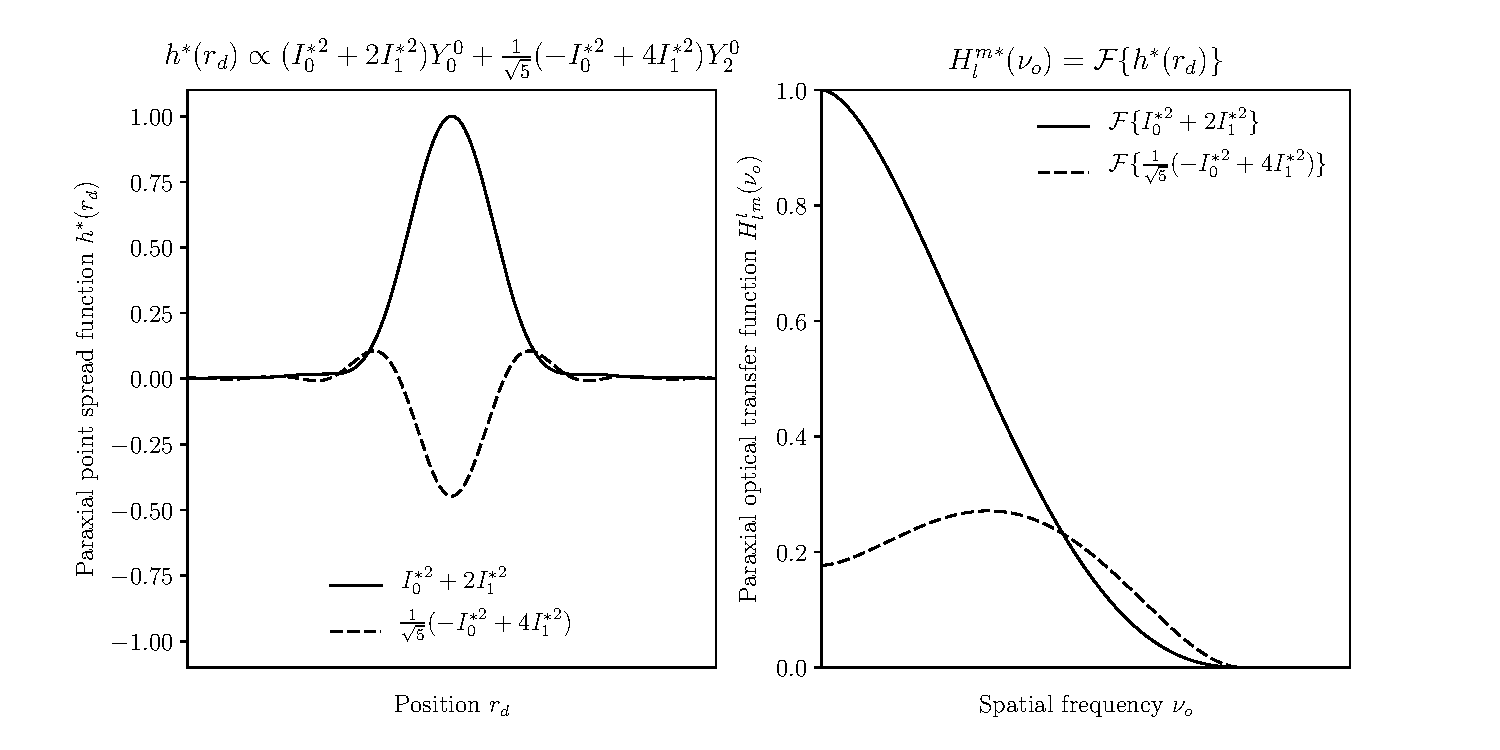
\includegraphics[width = 1.\textwidth]{../calculations/ft.pdf}
   \caption{\textbf{Left:} Paraxial spatio-angular point spread function for a
     single-view fluorescence microscope with NA=0.8. The solid line is the PSF
     for $y_0^0$ distributions and the dashed line is the PSF for $y_2^0$
     distributions. $y_2^0$ includes ``negative'' fluorophores, so it gives rise
     to a negative PSF. \textbf{Right:} Numerical paraxial spatio-angular
     optical transfer function for the same microscope. The $y_0^0$ term has a
     spatial low-pass response while the $y_2^0$ term has a spatial high-pass
     response. The relative sizes of the two terms is set by the NA---increasing
     the NA increases the relative size of the $y_0^2$ term. Vertical scaling is
     correct---horizontal scaling is in progress. The cutoff frequency is
     proportional to NA and is the same for both spherical harmonic terms.}
   \label{fig:para}
\end{figure}
    
\section{Conclusions}

TODO 

\bibliography{report}{}
\bibliographystyle{unsrt}

\appendix
\section{Paraxial optical transfer function in terms of elementary functions}
Our goal is to calculate the paraxial optical transfer function. We start by
plugging Eq. \ref{eq:kernel} into Eq. \ref{eq:ft}, using the paraxial
approximation, and constraining ourselves to the transverse plane
\begin{align}
  {H_l^m}^{(p)}(\bs{\nu}_o) = \int_{\mathbb{R}^2}d\mb{r}_o{} \int_{\mathbb{S}^2}d\so{}\ \left|\int_{\mathbb{R}^2} d\rb{}\, \mb{e}_b(\rb{}; \ro{}, \so{})\me^{-i (kn_t/f_t) \rb{} \cdot \rd{}}\right|^2
 y_l^m(\so{})\thinspace\me^{i 2\pi \ro{}\cdot\bs{\nu}_o}\label{eq:ft2}.
\end{align}
We change the order of the integrals
\begin{align}
  {H_l^m}^{(p)}(\bs{\nu}_o) = \int_{\mathbb{S}^2}d\so{}\ y_l^m(\so{}) \int_{\mathbb{R}^2}d\mb{r}_o\ \left|\int_{\mathbb{R}^2} d\rb{}\, \mb{e}_b(\rb{}; \ro{}, \so{})\me^{-i (kn_t/f_t) \rb{} \cdot \rd{}}\right|^2 \me^{i 2\pi \ro{}\cdot\bs{\nu}_o}, 
\end{align}
then apply the Wiener-Khinchin theorem
$\mathcal{F}\{|\mathcal{F}\{\mb{e}_b\}|^2\} = \mb{e}_b \star \mb{e}_b$ to find
that
\begin{align}
  H_l^m(\bs{\nu}_o) = \int_{\mathbb{S}^2}d\so{}\ y_l^m(\so{}) \left[\mb{e}_b \star \mb{e}_b\right](\bs{\nu}_o). 
\end{align}
The vector auto-correlation is given by
\begin{align}
[\mb{e}_b \star \mb{e}_b](\bs{\nu}_o) = \int_{\mathbb{R}^2}d\bs{r}_b \mb{e}_b^{T}(\bs{r}_b)\mb{e}_b(\bs{r}_b + \bs{\nu}_o),
\end{align}
where $\cdot^T$ denotes the transpose operator. 

\end{document}

